% !TEX TS-program = pdflatex
% !TEX encoding = UTF-8 Unicode

% This is a simple template for a LaTeX document using the "article" class.
% See "book", "report", "letter" for other types of document.

\documentclass[11pt]{report} % use larger type; default would be 10pt

\usepackage[utf8]{inputenc} % set input encoding (not needed with XeLaTeX)
\usepackage{amsmath,amssymb}
 \usepackage{mathtools}

\usepackage{graphicx}
 \usepackage{glossaries}
 
 \usepackage{longtable}
 
 \usepackage{graphicx} % support the \includegraphics command and options
 
 % \usepackage[parfill]{parskip} % Activate to begin paragraphs with an empty line rather than an indent
 
 %%% PACKAGES
 
 \usepackage{varwidth} % must be loaded after array
 
 
 \usepackage{verbatim} % adds environment for commenting out blocks of text & for better verbatim
 
 \usepackage{array} % for defining a new column type
 
% main git errors  handling https://www.javaprogramto.com/2021/11/error-failed-to-push-some-refs-to.html

 
\newcommand{\numberset}[1]{\mathbb{#1}}
\newcommand{\nat}{\numberset{N}}

\DeclarePairedDelimiterX{\Set}[2]\{\}{%
  \, #1 \;\delimsize\vert\; #2 \,
}

%%% Examples of Article customizations
% These packages are optional, depending whether you want the features they provide.
% See the LaTeX Companion or other references for full information.
\renewcommand{\arraystretch}{2}

\def\x#1{\texttt{\expandafter\string\csname#1\endcsname}&\expandafter$\csname#1\endcsname$}

 \newcommand{\stock}{\gets\mathrel{\mkern-2.4mu\mathop\square}}

\let\mtproforall\forall % just for the comparison
\let\mtproexists\exists % just for the comparison

\DeclareSymbolFont{CMsymbols}{OMS}{cmsy}{m}{n}
\SetSymbolFont{CMsymbols}{bold}{OMS}{cmsy}{b}{n}
\DeclareMathSymbol{\forall}{\mathord}{CMsymbols}{"38}
\DeclareMathSymbol{\exists}{\mathord}{CMsymbols}{"39}

\makeatletter
\providecommand*{\Dashv}{%
  \mathrel{%
    \mathpalette\@Dashv\vDash
  }%
}
\newcommand*{\@Dashv}[2]{%
  \reflectbox{$\m@th#1#2$}%
}
\makeatother


\newcolumntype{L}[1]{>{\flushleft\arraybackslash}p{#1}}



% Automatically added code


% \geometry{margin=2in} % for example, change the margins to 2 inches all round
% \geometry{landscape} % set up the page for landscape
%   read geometry.pdf for detailed page layout information


 

\title{Onderzoeksverslag sluizenpark \\
\large Automatisering van Sluizenpark in Nederland\\
    met Uppaal}
 

\author{Galvin Bartes}
%\date{} % Activate to display a given date or no date (if empty),
         % otherwise the current date is printed 

\begin{document}
	
%\newcolumntype{M}{>{\begin{varwidth}{4cm}}l<{\end{varwidth}}} %M is for Maximal column
	
\maketitle

\section{Samenvatting}
Het ministerie van verkeer en Waterstaat wil in het kader van het klimaatakkoord en onderzoek laten uitvoeren naar de staat van het sluizenpark in Nederland. Het onderzoek moet zich richten op het ontwerpen en ontwikkelen van een geautomatiseerd sluismodel dat geschikt is voor een brede toepassing. In het onderzoek moet naar voren komen wat de huidige staat is van de sluizen met oog op veiligheid, efficiëntie, capaciteit, onderhoud, duurzaamheid en automatisering. Het onderzoek geeft aan hoe een volledig model worden opgeleverd opdat ontwerp van verschillend volledig geautomatiseerde sluizen in de toekomst geautomatiseerd kunnen worden.  

\part{Onderzoek en ontwikkeling sluzienpark}

\chapter{Inleiding}

\subsubsection{Algemeen}

Het ministerie van verkeer en Waterstaat wil in het kader van het klimaatakkoord en onderzoek laten uitvoeren naar de staat van het sluizenpark in Nederland. Het onderzoek moet zich richten op het ontwerpen en ontwikkelen van een geautomatiseerd sluismodel dat geschikt is voor een brede toepassing. In het onderzoek moet naar voren komen wat de huidige staat is van de sluizen met oog op veiligheid, efficiëntie, capaciteit, onderhoud, duurzaamheid en automatisering. Het onderzoek geeft aan hoe een volledig model worden opgeleverd opdat ontwerp van verschillend volledig geautomatiseerde sluizen in de toekomst geautomatiseerd kunnen worden.  

\subsubsection{Probleemanalyse}

Na grondige analyse van het Nederlandse sluizenpark is gebleken dat renovatie van een groot aantal sluizen noodzakelijk is.  Uit een eerste verkenning is gebleken  dat het gecombineerd renoveren en automatiseren van het Nederlandsesluizenpark een aanzienlijke verbetering kan opleveren t.a.v. 
Op  het  ministerie  van  infrastructuur  enwaterstaat is helaas onvoldoende kennis van ict en systemen aanwezig om eenen ander uit te voeren 

\subsubsection{Waarom nu}
In  het  kader  van  het  onlangs  afgesloten  klimaatakkoord  heeft  de  Nederlandseoverheid  daarom  besloten  over  te  gaan  tot  een  ingrijpende  renovatie  van  dediverse  sluizen  die  ons  land  rijk  is.     

\subsubsection{Gewenst resultaat }

 
Wij vragen u een model (of een onderling samenhangend aantal modellen)aan  te  leveren,  opdat  ontwerpen  van  verschillende,  volledig  geautomatiseerdesluizen in de toekomst gerealiseerd kunnen worden. 
Zoals  gesteld  in  de  brief  is  het  de  bedoeling  dat  een  sluis  gemodelleerd  wordten  dat  bewezen  kan  worden  dat  de  te  bouwen  sluis  een  aantal  eigenschappenbezit.  
 
\subsubsection{Scope}
 
He gaat om het simuleren van een geautomatiseerde sluis. Wat voor type sluis wordt niet gemeld en ook niet uit welke onderdelen. Belangrijk is dat het model werkt en dat het voldoet aan de eisen die gebaseerd zijn op basis van literatuuronderzoek, observatie, interviews, brainstorming of een andere vorm van requirements elicitation.

\subsubsection{Onderzoeksvragen }






\begin{enumerate}
  \item Uit het onderzoek zal moeten blijken welke veiligheidseisen er zijn voor sluizen in nederland. 
  \item Daarnaast welke factoren een rol spelen in de duurzaamheid van het sluizenpark.  
  \item Hoe wordt de routinecontrole op de sluizen uitgevoerd?  
   \item Welke automatisering is mogelijk met oog op veiligheid, efficientie en capaciteit?  
    \item Welke criteria wegen zwaar in de ontwikkel- en onderhoudskosten van duurzame technologie?
\end{enumerate}


\newpage
\subsubsection{Vooronderzoek }

\paragraph{Systeem versus softwareengineering}


\paragraph{requirements}
requirements versus specificaties 
requirements are a usable representation of a need.

Specificaties
The software requirement specificatie bevat een omschrijving van functies en mogelijkheden die het product moet kunnen bieden. In de specificatie wordt ook vastgelegd welke beperkingen en aannames worden gedaan. De specificatie wordt soms verduidelijks aan de hand van use cases en user stories.




The document also defines constraints and assumptions. The SRS can be a single document communicating functional requirements or it may accompany other software documentation like user stories and use cases.
type requirements 

hoe requirements elicitation toepassen 
Creating requirements is a complex task as it includes a set of processes such as elicitation, analysis, specification, validation, and management. In this article, we’ll discuss the main types of requirements for software products and provide a number of recommendations for their use.

Het iseen manier van onderzoek en ontdekken van de requirements van een systeem van de gebruikers, klanten en andere stakeholders.
Dit kan uitgevoerd worden door:
Brainstorming
Document analyse
Focus group
Interface analyse
Interviews observaties
Process modellering
Prototypingh
Requirement workshops
surveys/questionaiire

\paragraph{specificaties}

\paragraph{functioneel vs niiet-functioneel}


\subparagraph{subparagraph}


\paragraph{Automatiseringsparadox}



\paragraph{Rampen}



\subparagraph{subparagraph}
therac-25 
Softwarefout uit zich als hardwarefout de klachtafhandeling geen onderzoek geen second opinion is prioriteit wel 
gechecked na onderzoek bellen en geen prioriteit aanwezig te zijn alleen importeurs en fabriken mogen fouten 
in frabrieksinstellingen rapporteren 
Therac25 Systeem ligt plat veel voorkomende eror stdaardafhandeling om de error te verwerpen resultaat: 
de patient kreeg overdosis patient overleden onderzoek opgestart, stuatie niet reproduceerbar foutmarkering: 
gezien als uitzonderlijk, software aanpassing van groote magnitude 5; de oorzaak was waarschijlijk mechanisch 
maar neit vastgesteld; conceptueel odel niet aangepast probleemclassicificatie door autorititen het probleem 
en de impact daarvan anar beneden bijgesteld AEFL doe gedeeltelijke aanpassing om hardware na berisping 
Canadese autoriteit 
Derde patient overleden door eythema AECL wijst alle doodsoorzaken af AECL beweert dat geen vergeli- 
jkbare voorvalle bij andere machines of patienten zijn voorgekomen geen vervolgonderzoek vanwege garanties 
bedrijf gaat uit van geen mogelijke functionele fout 
vierde patient overleden aan overdodis ontstaan door bug in software onjuiste aanduiding bij de foutmelding 
verkeerde reactie/invoer ddoor operator communicatie tussen patient en operator werd onvoldoende gemon- 
itorred ( apparatuur niet aangesloten, en audio monitor kapot) engineer van AECL stelt geen fouten vast 
Engineer AECl kan fout niet reproduceren Geen communicate tussen bedrijf en uitgezonden technisci over 
vergelijkbare probleemgevallen 
vijfde geval malfunction 54 leidt tot overdosis en de dood fout gereproduceerd door operator bedrijf fout 
was daa entryspeed herpublicatie van de ongevallen en de eerdere ongevallen in de meia apparaat wel nog in 
gebruik genomen niet handig, waarschuwingsberichten en aanwijzingen voor een bugfix naar de gebruikers door 
druk van fda is bedrijf op zoek gegaan naar permanente oplossing 
zesde geval software fout door softwarefout otntstaat lightstruct .. op de patient na onderzoek door AECL 
blijkt niet alleen hardware de oorzak gebruikers direct geinformeerd oplossing gevonden, media ingeschakeld om 

transparantie af te dwingen door de gebruikersgroep en de FDA AECL gedwongen functionaliteit aan te passen 
Engineers hebben meer studie moeten maken van gebruikte technologie en onderhoudbaarheid daarvan 


mode confusion 
Mode confusion treed op als geobserveerd gedrag van een technisch systeem niet past in het gedragspatroon 
dat de gebruiker in zijn beeldvorming heeft en ook niet met voorstellingsvermogen kan bevatten 

\subparagraph{automatiseringsparadox }
Gemak dient de mens. Als er veel energie wordt gestoken in de ontwikkeling van hulmiddelen die taken van 
werknemers overemen heeft dat tot resultaat dat veel productieprocessen worden geautomatiseerd. De vraag is 
dan of vanuit mechnisch wereldpunt de robot niet de rol van de mens overneemt en of de mens nog de kwaliteiten 
heeft om het werk zelf te doen 

\subparagraph{functioneel vs non-functionele eisen }
 We kunnen requirements onderverdelen in functionele en niet-functionele nrequirements

Functional requirements define what a product must do, what its features and functions are.


Nonfunctional requirements describe the general properties of a system. They are also known as quality attributes.
https://www.altexsoft.com/blog/business/functional-and-non-functional-requirements-specification-and-types/

\subparagraph{Ramp schietpartij militair ossendrecht }
\subparagraph{ramp mali missie }
\subparagraph{molukse treinkaping }
\subparagraph{vuurwerkramp in enschede }
\subparagraph{elektriciteitsnet in oekraine }
\subparagraph{explosie in libabon, beirut }
\subparagraph{explosie tanjin china }
\subparagraph{bijlmerramp }
\subparagraph{slm ramp }
\subparagraph{Ethiopian Airlines Flight 302 }

\subparagraph{stint ongeluk }
\subparagraph{tjernobyl  }
\subparagraph{tesla crash  }
\subparagraph{Ramp turkish airlines  }
\subparagraph{slm ramp }



\paragraph{Previous work}





\paragraph{Methdodologie}

Om een prototypoe op te leveren zinj de volgende technieken gebruikt

 \begin{enumerate}
	\item Deskresearch
	\item Sketching
	\item Prototyping
\end{enumerate}

\subparagraph{Deskresearch}
Er is een deskresearch uitgevoerd naar de verschillende sluzien, bedieningstijden, gautomatiseerde sluizen, rampen die te maken hebben met controle systemen en de omgevingsvariabelen die een rol spelen bij automatisering.

%%%%%%%%%%%%%%%%%%%%%%%%%%%%%%%%%%%%%%%%%%%%%%%%%%%%%%%%%%%%%%%%%%%%%%%%%


\begin{frame}{Literature Review}
	\begin{table}[htbp]
		\footnotesize
		
		\centering
		\begin{tabular}{|c|c|p{2in}|c|c|}\hline
			S.no&Author&Title&Findings&Gap in literature\\\hline
			S.no&Author&wanrooy \textunderscore vab1991a.pdf&Findings&Gap in literature\\\hline
			S.no&Author&wa3300-bezuien2000(1).pdf&Findings&Gap in literature\\\hline
			S.no&Author&Title&Findings&Gap in literature\\\hline
			S.no&Author&Title&Findings&Gap in literature\\\hline
			S.no&Author&rapport-veiligheid-van-op-afstand-bediende-burggen.pd&Findings&Gap in literature\\\hline
			S.no&Author&pronk.pdf&Findings&Gap in literature\\\hline
			S.no&Author&Olieman1987a.pdf&Findings&Gap in literature\\\hline
			S.no&Author&richtlijnen-vaarwegen-2020.pdf&Findings&Gap in literature\\\hline
			S.no&Author&richtlijnen-vaarwegen-2017 \textunderscore tcm21-127359(1).pdf&Findings&Gap in literature\\\hline
			S.no&Author&Olieman1987a.pdf&Findings&Gap in literature\\\hline
			S.no&Author&Meijer1980b.pdf&Findings&Gap in literature\\\hline
			S.no&Author&Meijer1980c.pdf&Findings&Gap in literature\\\hline
			S.no&Author&kst-31200-A-80-b2.pdf&Findings&Gap in literature\\\hline
			S.no&Author&duurzaamheid \textunderscore bij \textunderscore de \textunderscore ontwikkeling \textunderscore van \textunderscore reevesluis.pdf&Findings&Gap in literature\\\hline
			S.no&Author&De \textunderscore deltawerken \textunderscore Cultuurhistorie \textunderscore ontwerpgeschiedenis \textunderscore web-A.pdf&Findings&Gap in literature\\\hline
			S.no&Author&wa3300-Bezuijen2000.pdf&Findings&Gap in literature\\\hline
			S.no&Author&Sander van Alphen Haalbaarheidsstudie naar grote sluisdeuren uitgevoerd in hogesterktebeton.pdf&Findings&Gap in literature\\\hline
			S.no&Author&Dalmeijer1994a.pdf&Findings&Gap in literature\\\hline
			S.no&Author&Dalmeijer1994b.pdf&Findings&Gap in literature\\\hline
			S.no&Author&Dalmeijer1994c.pdf&Findings&Gap in literature\\\hline
			S.no&Author&ceg \textunderscore pruijssers \textunderscore 1982.pdf&Findings&Gap in literature\\\hline
			S.no&Author&Capaciteitsanalyse \textunderscore van \textunderscore de \textunderscore prinses\textunderscore margrietsluis \textunderscore in \textunderscore lemmer \textunderscore - \textunderscore Marc \textunderscore Lamboo.pdf&Findings&Gap in literature\\\hline
			S.no&Author&Boer1979a.pdf&Findings&Gap in literature\\\hline
			S.no&Author&bijlagerapport \textunderscore c \textunderscore - \textunderscore analyse \textunderscore geavanceerd-definitief \textunderscore v1 \textunderscore 0.pdf&Findings&Gap in literature\\\hline
			S.no&Author&Bijl1988a.pdf&Findings&Gap in literature\\\hline
			S.no&Author&Bentum1978a.pdf&Findings&Gap in literature\\\hline
			S.no&Author&Alphen.pdf&Findings&Gap in literature\\\hline
			S.no&Author&Abbenhuis1975a.pdf&Findings&Gap in literature\\\hline
			S.no&Author&Abbenhuis1974a.pdf&Findings&Gap in literature\\\hline
			S.no&Author&https://wiki.woudagemaal.nl/w/index.php/Sluizen&Findings&Gap in literature\\\hline
			S.no&Author&Title&Findings&Gap in literature\\\hline
		 		
		\end{tabular}
	\end{table}
	
\end{frame}
%%%%%%%%%%%%%%%%%%%%%%%%%%%%%%%%%%%%%%%%%%%%%%%%%%%%%%%%%%%%%%%%%


\begin{longtable}{|c|c|c|c|c|}
	\caption{A simple longtable example}\\
	\hline
	\textbf{SBNO} & \textbf{Author} & \textbf{Title} & \textbf{Findings} & \textbf{Gap in literature} \\
	\hline
	\endfirsthead
	\multicolumn{5}{c}%
	{\tablename\ \thetable\ -- \textit{Continued from previous page}} \\
	\hline
	\textbf{SBNO} & \textbf{Author} & \textbf{Title} & \textbf{Findings} & \textbf{Gap in literature} \\
	\hline
	\endhead
	\hline \multicolumn{5}{r}{\textit{Continued on next page}} \\
	\endfoot
	\hline
	\endlastfoot
	1 & 2 & 3 & 4 &5 \\ \hline	
		1 & 2 & 3 & 4 &5 \\ \hline	
			1 & 2 & 3 & 4 &5 \\ \hline	
				1 & 2 & 3 & 4 &5 \\ \hline	
 
\end{longtable}

%%%%%%%%%%%%%%%%%%%%%%%%%%%%%%%%%%%%%%%%%%%%%%%%%%%%%%%%%%%%%%%%%

\subparagraph{Sketching}

Er zijn met google search engine afbeeldingen gezocht van sluizen om een overzicht te krijgen van de  verschillen.

\subparagraph{prototyping}
om een voledig werkend model van een geautomatiseerde sluis te kunnen simuleren is met simulatiesoftware en CTL-logica een model geimplementeerd

\paragraph{leeswijzer}

\newpage

\chapter{Uitvoering}

\section{Requirementanalyse}

\subsection{Inleiding}
Een requirement is een opdracht gedefineerd door een klant. In requirement komt naar voren wat er specifiek wordt gevaard, voor wie het is bedoeld, of het meetbaar is,  de acceptatieeisen,een realistische perceptie  het doel of gewenst resultaat en binnen welke tijdseenheden het moet worden gerealiseerd.

\subsection{Middenstuk}

\subsection{Resultaat}

 \begin{enumerate}
 	\item Een schip kan kan worden gesignalererd voor invaren en uitvaren. 
	\item Een sluiskolk heeft sluisdeuren.  
	\item De sluis kan het waterpeil in de sluiskolk aanpassen aan de omgeving. 
    \item Er is een controller die het verkeer regelt tussen de subonderdelen in de sluis zelf en die tevens de communicatie met de buitenwereld onderhoudt dmv signalering.
\end{enumerate}




\subsubsection{Model}

In een real-life omgeving kan rekening worden gehouden met de volgende aspecten uit de omgeving
storm
ijs
diepte
windkracht
andere schepen
eigen vermogen

\subsubsection{Aankomst, uitvoering, vrijgave}


\subsubsection{ontwerp}

 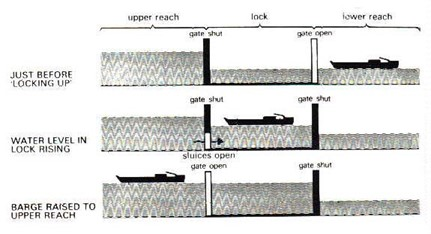
\includegraphics[scale=0.65]{sluismodel.jpg}
 
 \subsubsection{Onderdelen}
 Op basis van de schets kunnen we vaststellen dat een sluismodel uit de volgende onderdelen bestaat.
 
 \begin{enumerate}
 	\item Een tweetal sluisdeuren. 
 	\item Een sluiskolk waarin de schepen in- enuitvaren
 	\item een stoplicht om een signaal af te geven voor invaren en uitvaren.
 	\item Een nivelleermachine zorgt ervoor dat het water in de sluis op het gewenste niveau wordt gebracht
 	\item Een control-system dat ervoor zorgt dat de opdrachten van de sluisbeheerder (geautomatiseerd) worden uitgevoerd
 \end{enumerate}
\subsubsection{Werking}

Een schip komt aanvaren en meld zich aan bij de sluismeester. De sluismeester geeft een signaal aan het controlsystem voor het openen van de sluisdeuren, nadat geccontroleerd is of de nivelleermachine al klaar is. Als er ruimte is voor een invarend schip mag het schip dat zoich heeft aangemeld en toestemming heeft  in de sluis varen. Op het moment dat de sluis vol is gaan de sluisdeuren dicht. Eenmaal afgesloten kan de nivelleermachine beginnen om het water in de sluiskolk op het gewenste waterpeil te brengen. Als dit nivelleerprces is afgerond geeft  het controlsystem daan da de sleusdeuren open kunnen.  Als de sleusdeuren open zijn en het uitvaarsignaal is op groen dan moet het schip in de sluis de sluis uitvaren.
 \paragraph{extra cases}
 Uit het zojuist genoemnde scenario valt het volgende op te maken.
  \begin{enumerate}
 	\item Een schip geeft een signaal aan een sluismeester.
 	\item Er wordt gekeken of er wel plek is in de sluis .
 	\item Er wordt gekeken of de nivelleermachine is afgerond.
 	\item Er wordt gekeken wat het niveo van de waterpeil in de sluiskolk is.
 	\item Er wordt gekeken of de sluisdeuren gereed zijn voor invarende schepen.
 \end{enumerate}
 \paragraph{Aandachtspunten}
   \begin{enumerate}
 	\item Voorrang tussen schepen onderling in de sluis?
 	\item Hoe lang mag een schip zich in de sluis bevinden?
 \end{enumerate} 

%%%%%%%%%%%%%%%%%%%%%%%%%%%%%%%%%%%%%%%%%%%%%%%%%%%%%%%%%%%%%%%%%
\section{Een voorbeeld}

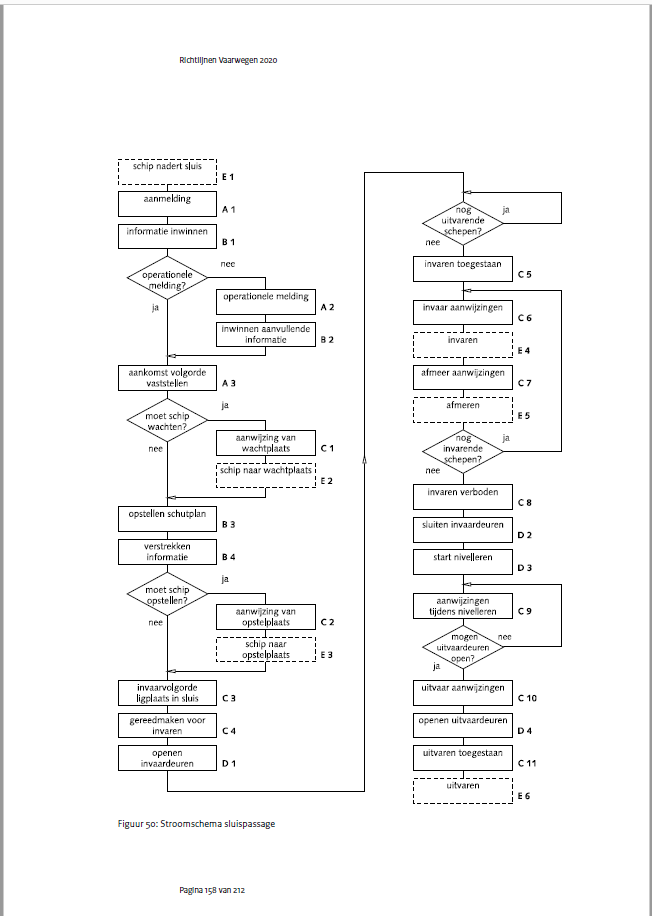
\includegraphics[scale=0.65]{sluispassage.png}

\paragraph{Vooraanmelding}


\paragraph{informatie inwinnen}


\paragraph{operationele melding}


\paragraph{aankomst volgorde}

\paragraph{aanwijzen wachtplaats}


\paragraph{verstrekken informatie}


\paragraph{aanwijzen opstelplaats}

\paragraph{opstellen schutproces}


\paragraph{verstrekken informatie}


\paragraph{invaarvolgorde en ligplaats in sluis}

\paragraph{gereedmaken voor invaren}



\paragraph{openen invaardeuren}




\paragraph{invaren toegestaan}

\paragraph{aanwijzingen voor invaren}
\paragraph{aanwijzingen tijdens afmeren}

\paragraph{invaren verboden}

\paragraph{sluiten invaardeuren}

\paragraph{start nivelleren}

\paragraph{aanzwijzingen voor uitvaren}
\paragraph{openen uitvaardewuren}

\paragraph{uitvaren toegestaan}




\paragraph{brainstorm 22-5-2022}

\subparagraph{invaardeuren en uitvaardeuren}
Gaan we uit van binnendeuren en buitendeuren? Er ontstaat dan een extra ruimte in de sluis. Hoeveel schepen kunnen in deze ruimte? Wat is de maximale wachtreij in deze ruimte en wat zijn de verkeersregels in deze nruimte?
\subparagraph{invaarstoplicht en uitvaarstoplicht}
Als invaren is toegestaan hoe wordt dit dan doorgegeven aan de schepen in de sluis? moeten zij dan uit zichzelf wachten of krijgen zij een signaal dat zij wewl/niet mogen uitvaren? En moeten zij dan kiezen voor links, midden of rechts? Of maakt dat allemaal niets uit?

\subparagraph{invaarwachtrij en uitvaarwachtrij}
Als er meerder schepen in een sluiskolk zitten moet het systeem dan rekeneing houden met het schip dat als eerste is ingevaren en/of het langst in de sluis zit?


%%%%%%%%%%%%%%%%%%%%%%%%%%%%%%%%%%%%%%%%%%%%%%%%%%%%%%%%%%%%%%%%%

\section{Uppaal kripke structuren}


\subsubsection{templates}

\paragraph{Schip}

\paragraph{Sluis}


\paragraph{Aanvoer}


\paragraph{Afvoer}

\paragraph{Pomp}

\paragraph{Pompbediening}


\paragraph{Stoplicht}

\paragraph{Deur}


 \subparagraph{case}
Als een schip van rechts binnen komt en sluisdeuren zijn dicht dan moet het stoplicht op rood, de pomnp in transitie van laag naar hoog en niet andersom

 \subparagraph{case}
 Voor invaren geldt altijd: waterlevel, pomp uit, sluisdeuren open en stoplicht op groen
 
  \subparagraph{case}
  uitvarenden hebben voorang op invarenden
  
   \subparagraph{case}
   Voor invarenden geldt pomp uit, sleusdeur open en stoplicht op groen
    \subparagraph{case}
    voor nivelleren geldt pomp is aan, sluisduren zijn doicht en het stoplicht is op rood
     \subparagraph{case}
     Als een schip vertrekt dan zijn altijd, sleusdeuren open, waterlevel gereed op niveau 5 of 0 en stoplicht direct op groen
      \subparagraph{case}
      urgent locations; het is niet mogelijk om hier te wachten
       \subparagraph{case}
       urgent syn; een synchronisatie moet direct worden uitgevoerd als de guards geldig zijn
       
        \subparagraph{case}
        als een schip binnen is, en er zijn wachtende schepen, dan moet het stoplicht via oranje naar rood
         \subparagraph{case}
         committed; als deze staat actief is dan wordt de eerst volgende transitie uitaande van deze state
          \subparagraph{case}
          als een schjip binnen vaart mnoiet hij ook eft binnen zijn en niet binnenvaren, dit geldt ook voor sluisdeuren en pompen dus deze zijn committed.
           \subparagraph{case}
           
            \subparagraph{case}
            
             \subparagraph{case}
             
\paragraph{Parallele compositie}


\paragraph{Parallele compositie}

\subsubsection{Modeleigenschappel}
\paragraph{Parallele compositie}
Om een sluispark te kunnen modelleren meerdere templates die de verschillende abstracties van het systeem aantonen.

\paragraph{Synchronisatgie}
Zorgt ervoor dat  een transitie die genomen worden in de ene kripke tructuur op hetzelfde moment wordt opgenomen in een andere kripke structuur.



\chapter{CTL logica}

 
\section{Doel van de test}
\subsection{Wat wordt getest en hoe}
	

\subsection{toetsen met queries}
\begin{tabular}[t]{rl|rl}%
    \x{lnot}    & \multicolumn{2}{c}{none}\\
    \x{square}  & \x{lozenge}\\
    \x{vee}     & \x{wedge}\\
    \x{vdash}   & \x{models}\\
\end{tabular}




\subsection{Operator: AG}
Voor alle paden


\subsection{Operator: EG}
Uiteindelijk geldt er een pad waarvoor geldt

\subsection{Operator: AF}
Voor alle paden/richtingen vroeg of laat
\subsection{Operator: EF}
Er is een pad
\subsection{Operator: AX}
Alle opvolgende toestanden

~\cite{locke_2020}
\subsection{Operator: EX}
Er bestaat vanaf de volgende minstens 1 state waarvoor geldt
\subsection{Operator: p U q}
Er geldt p tot q
~\cite{gnsguides}
\subsection{Operator: p R q}
q moet waar zijn totdat en inclusief de situatie dat p voor het eerst waar is, als p niet geldig is, dan moet q vooraltjd geldig zijn
\subsection{Fairness}
AG(AF(p))
\begin{verbatim}
	In welke staat de automaat zich ook bevindt, in alle richtingen kom je vroeg of laat een state tegen, waarin p geldig is.
\end{verbatim}
\subsection{Liveness}
\begin{verbatim}
	Altijd en overal geldt: Als p geldt dan geldt vroeg of laat q
	Ookal treedt p nooit p volgens de logica klopt het dan dat q volgt uit p.
	In een situatie, waarin p nooit optreedt, spreekt men van een
	vacuous truth.
\end{verbatim}


\begin{center}
	\begin{tabular}{| l | c || r | }
		\hline
		1 &A[] !deadlock  &  TRUE \\ \hline
		2 & A[] not (Sluis.Tussenstop5 \&\& Deur.Klaar\_voor\_uitvaart)  &  Disconnected \\ \hline
		3 & A[]  (Sluis.Voorbereiden imply Deur.Dicht)   &  TRUE\\   \hline
		4 &A[]  (Deur.Dicht imply Counter==0)   & TRUE  \\   \hline
		5 & A[]  (Buitenstoplicht.Groen imply invaren\_allowed==true)  &  TRUE \\ \hline
		6 & A[] ! (Binnenstoplicht.Groen imply invaren\_allowed==false)  & FALSE \\ \hline
		7 & A[]  (globale\_tijd>30)   &  FALSE\\    \hline
		8 & E<>  (Schip.Stoppen and (Counter >5))   & Ship not a structure  \\   \hline
		9 & A[] (Schip.Vertrekken imply Sluisdeur.Dicht)  &  -  \\   \hline
		\hline
	\end{tabular}
\end{center}


\begin{verbatim}
	
	Queries
	Sluis.Draining-->Deuren.laag_open
	Deuren.laag_open-->Stoplicht.Green
	E<> (Ship.ship_can_move&&Stoplicht.Green)
	A[] not (Stoplicht.Green && not (Deuren.hoog_open||Deuren.laag_open||Deuren.stopgaplow1||Deuren.stopgaplow2||Deuren.stopgaphigh1||Deuren.stopgaphigh2))
	A[] not ((Deuren.hoog_open||Deuren.laag_open||Deuren.Opening_laag||Deuren.Opening_hoog||Deuren.Closing_hoog||Deuren.Closing_laag) && (Sluis.Draining||Sluis.Filling||Sluis.draining2||Sluis.Filling2))
	Sensor.Wait-->Sensor.Wait
	Stoplicht.Green-->Stoplicht.Green
	(Deuren.hoog_open||Deuren.laag_open)-->(Deuren.laag_open||Deuren.hoog_open)
	Deuren.laag_open-->Deuren.Closed
	Deuren.hoog_open-->Deuren.Closed
	Deuren.Closed-->Stoplicht.Red
	Ship.ship_can_move-->Deuren.Closed
	Deuren.hoog_open-->Stoplicht.Green
	Ship.ship_can_move-->Stoplicht.Green
	A[] not (Deuren.laag_open && Deuren.hoog_open)
	Ship.ship_can_move-->Ship.ship_can_move
	A[] not (Deuren.laag_open && Sluis.water != Sluis.water_laag)
	A[] not (Deuren.hoog_open && Sluis.water != Sluis.water_hoog)
	A[]not deadlock
	
	Project declaraties
	//Declarations
	
	chan boot_hoog;
	chan boot_laag;
	chan changedoor_low;
	chan changedoor_high;
	chan ship_moves;
	chan ship_abletomove;
	chan changelight;
	
	\\Sluis declaraties
	const int water_laag=0;
	const int water_hoog=10;
	const int water_median=(water_hoog+water_laag)/2;
	int[water_laag,water_hoog] water=water_median;
	clock x;
	\\Stoplicht declaraties
	
	\\Ship declaraties
	clock x;
	\\Sensor declaraties
	
	\\Deuren declaraties
	bool stoplicht_hoog=false;
	bool stoplicht_laag=false;
	clock x;
	
	
	\\System declaraties
	system Deuren,Sensor,Sluis,Ship,Stoplicht;
	
	
	Uitleg
	Als het schip boven is, dan is waterlvel gelijk aan hoog, filling valve is dicht, lower gates zijn gesloten, uppergates zijn open,empty valve is dicht. 
	Schip is in waterlock, waterlevel is hoog, filling valve is dicht, lower gates gesloten, upper gates gesloten, empty valve is open. 
	Schip is dan laag, waterlevel gelijk aan laag, filling valve is dicht, lowergates zijn open, uppergates zijn dicht, empty valve is dicht.
	AtArrivalHigh
	
	AtArrivalLow
	Als schip beneden is dan is waterlevel gelijk aan laag, filling valve is dicht, lower gates zijn open, upper gates zijn dicht, empty valve is open. 
	Schip is in water lock, waterlevel is laag, flilling valve is open, lower gates zijn gesloten, upper gates zij gesloten, empty valve is dicht,. 
	Schip is dan hoog, waterlevel is gelijk aan hoog, filling valve is dicht, uppergates zijn open, lowergates zijn dicht, filling valve is dicht
	
	
	
\end{verbatim}
\begin{gather*}
D=\Set{x\in\nat}{1\le x\le 100}\\
D=\Set[\big]{x\in\nat}{1\le x\le 100}\\
D=\Set[\Big]{x\in\nat}{1\le x\le 100}\\
D=\Set[\bigg]{x\in\nat}{1\le x\le 100}\\
D=\Set[\Bigg]{x\in\nat}{1\le x\le 100}\\
D=\Set*{x\in\nat}{1\le x\le \frac{200}{2}}
\end{gather*}

\begin{align}
    \alpha &= \beta + \gamma * \lambda \\
     \alpha &= \beta + \gamma * \lambda \\
      \alpha &= \beta + \gamma * \lambda \\
    \theta &= \frac{\alpha}{4}
\end{align} 

%  https://www.stat.cmu.edu/~brian/latex/symbols/symbols.html
% https://tex.loria.fr/ctan-doc/macros/latex/doc/html/fntguide/node18.html
% https://observablehq.com/@s-haensch/latex-notation
% http://tdc-www.harvard.edu/tdcprop1/help/symbols/
% http://new.math.uiuc.edu/oldnew/netgeom/advice/to-texpad.html
% https://www.overleaf.com/learn/latex/List_of_Greek_letters_and_math_symbols
% https://jblevins.org/log/greek
% https://latex-tutorial.com/symbols/greek-alphabet/
% https://latex-programming.fandom.com/wiki/List_of_LaTeX_symbols
% https://physicsanduniverse.com/latex-symbols-and-using-them-to-write-equations/
% http://tug.ctan.org/info/symbols/comprehensive/symbols-a4.pdf
% https://tex.stackexchange.com/questions/99772/how-to-insert-greek-letters-having-trouble-with-greekletter
% https://texblog.org/2012/03/15/greek-letters-in-text-without-changing-to-math-mode/
% https://www.avantixlearning.ca/microsoft-word/how-to-insert-greek-letters-or-symbols-in-microsoft-word/
%
%
%




$S is a set of finite states$\\
$S0 \subseteq S is de set van initiele statess$ \\
$S0 \subseteq S xS  is een transitie relatie die totaal moet zij, dat betekent, dat voor elke state s \in S er een stats is s' \in S zodat R(s,s')$
$L\stock a$

$\forall x\,\exists y \implies $

$\mtproforall x\,\mtproexists y \cap \subset \in \vee \diamondsuit \dashv \ni \pm$


\subsubsection{onderdeleel van de test}
\paragraph{resultaat}
\subparagraph{verklareing}


\subsection{liveness}


\subsection{safety}


\subsection{zeno vrij}
Geen enkele state kan oneindig een transitie uitvoeren. Elke state heeft een uitgaande transitie.

\subsection{deadlocks}

\chapter{Conclusie}




\chapter{Discussie}

\subsection{Future work}
\subsubsection{Hoogte waterniveau}

\subsubsection{type deuren naar waterniveau}
De sluis kan ook rekening houden met waterniveau van hoog naar laag.
Als een schip naar binnen vaart moet de sluis weten welk schip ook werer naar buiten vaart en aan welke kant.

\subsubsection{voorrang uitvarend op invarend}
Als een schip uitvaart komt er een moment dat een sluis ruimte vrij heeft. Voordat de sluisdeur sluit nadat eenschip is vertrokken kan er nog een polling worden gedaan naar alle schepen in de buurt om te zien of deze willen en kunnen invaren.

\subsubsection{stoplicht invarend en stoplicht uitvarend}
Een handige functionaliteit is dat voor invarende schepen er een stoplicht is en voor uitvarende schepen. Anders ontstaat er een probleem van collission. 

\subsubsection{Volgorde}
Kunnen aantonen dat schepen kunnen worden behandeld met voorkeur, wie het eerst komt die het eerste in behandeling wordt genomen.

\chapter{Relevante begrippen}


 

\part{reflectie, projectaanpak en ontwikkeling}


Aanleiding
De inspectie van het onderwijs

De inspectie van het onderwijs voorziet risico's bij bvassischool Caleides en voert daarom op die schpool een risicoanalyse uit. Het rapport is een verslag van deze analyse en de resultaten daarvan.

Doel van het rapport
Tekstdoel; het rapport heeft tot doel een oordeel te geven over de kwaliteit van het onderwijs, in het bijzonder van de kwaliteitsindicatoren 'Opbrengsten', 'Schoolklimaat' en 'leeropbrengst'. De inspectie geeft geen advies.
Doel van de risicoanalyse. De inspectie wil de kwaliteit  van het onderwijs handhAVEN. hAAR MISSIE IS 'effectief toezicht  voor beter onderwijs'


Wie is de lezer
Het rapport is bestewmd voor het bestuur van de school en voor alle medewerkeras. Daarnaast wordt het rapport gelezen door kritische ouders. Een inspectierapport valt onder de Wet Openbaarheid bestuur en dat ias openbaar. Hieronder staaat wat het betekent voort de tekast in het rapport.

Het bestuur en de medewerkers zullen bij een onvoldoende oordeel precies wille n weten hoe dat komt. Zij willen weten;
wat de  argumenten zijn voor de tekst in het rapport
waar die argumenten op gebaseerd zijn; welke toetsingscriteria en welk bewijsmateriaal


De ouders willen snel kunnen kunnen zien wat het oordeel is van de inpectie en hoe de schoolo op bepaalde normen scoort. Zij willen;
een scanbaar rapport; waarin ze snel kunnen vinden wat ze zoeken
de tekst kunnen snappen
helder hennen waar toetscriteria voor staan; wat betekent bijvoorbeeld schoolklimaat


Kaders voor deze tekst: de toetscriteria. om neen oordeel te geven over de kwaliteit van het onderwijs, moeten de toetscriteria duidelijk zijn. De inspectie heeft die scherp gredefoinieerd. Zie het toetsingskder op de website vam de inspectie.

De hoofdvraagw waarop het rapport antwoordt geeft: leeft basischoool Caleidos de wet- en regelgeving na die de overheid voor het primair onderwijs heeft vastgesteld? het antwoord=het oordeel= de conclusie


Mogelijke subvragen:
over wlke school gaat het en waarom is daar een risicoanalys euitgevoerd?
Wat zijn de normen en naar welke toetscriteria zijn deze vertaaldd?
Hoe scoort de school op die toetscriteria en de normen?
Wat zijn de verschillen tussen de gewenste situatie bij antwoord c en de weke;lijke situatie?
Hoe  verklaart het schooolbestuur die verschillen?

Planning;
het onderzoek vindt plaats in maart. begin april presenteert de inspectie de resultaten aan het bestuur. Voior de meivakantie moet  het rapport bij het schoolbestuur liggen. Noteer eventueel aanvullend een deelplanning; wie doet het onderzoek; wanneer zijn de resultaten gereed; wie leest het conceptrapport

GHoofdtekst is 4 paginas
Onderliggend verslag van onderzoek is 20 pagina's




\chapter{managementsamenvatting}
managementsamenvatting
Inleiding
aanleiding, context, hoofdvraag van het rapport. Is de aanpak van het ziekteverzuim effectief?

Doelen van de aanpak ziekteverzuim
Wat is de gewenste situatie?
Wat is de huidige situatie?

Toetsingscriteria
Hoe is de huidige situatie getoetst?
Criterium 1
Criterium 2

Balans 
hoe zwaar wegen de uitkomsten

Conclusie
Wat is dus, gezien  het bovenstaande, het antwoord op de hoofdvraag van het rapport?






\end{document}
